\documentclass[10pt,a4paper]{article}
\usepackage[utf8]{inputenc}
\usepackage[german]{babel}
\usepackage{amsmath}
\usepackage{amsfonts}
\usepackage{amssymb}
\usepackage{siunitx}
\usepackage[left=2cm,right=2cm,top=2cm,bottom=2cm]{geometry}
\usepackage{wrapfig}
\usepackage{graphicx}
\usepackage[outdir=./figures/]{epstopdf}
\usepackage[colorlinks]{hyperref}
\usepackage{xcolor}
\usepackage{listings}
\lstset{basicstyle=\ttfamily,
  showstringspaces=false,
  numberstyle=\color{green},
  commentstyle=\color{red},
  keywordstyle=\color{blue},
  morekeywords={*, ./numerik_6}
}

\author{Christopher Deutsch}
\title{Übungsblatt 6: Numerische Methoden der Physik}
\begin{document}
\maketitle
\setcounter{section}{5}

\section{Doppelpendel}
\subsection{Physikalischer Hintergrund}
\subsubsection{Einführung}
\begin{wrapfigure}[18]{R}[1pt]{0.35\textwidth}
\centering
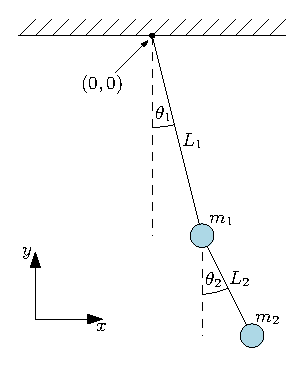
\includegraphics[width=0.33\textwidth]{./figures/pendel.eps}
\caption{Doppelpendel}
\label{fig:doppelpendel}
\end{wrapfigure}
In dieser Aufgabe soll ein Doppelpendel wie in Abbildung \ref{fig:doppelpendel} betrachtet werden. Dabei wurden die beiden Punktmassen $m_1$ und $m_2$ über eine starren, massenlosen Stab der Länge $L_2$ verbunden. Weiterhin ist die Masse $m_1$ reibungsfrei mit der Decke verbunden. Im Folgenden soll das System mit dem Lagrange-Formalismus beschrieben werden, um zwei Bewegungsgleichungen für die Winkel $\theta_1$ und $\theta_2$ zu erhalten. Schließlich werden die zwei Bewegungsgleichungen zweiter Ordnung in ein Differentialgleichungssystem erster Ordnung transformiert, welches dann mit dem Runge-Kutta-Verfahren vierter Ordnung auf einem endlichen Zeitintervall gelöst werden kann. Zuletzt soll das Verhalten des Systems bei verschiedenen Anfangsbedingungen untersucht werden.

\subsubsection{Lagrange-Funktion und Bewegungsgleichungen}
\label{sssec:Lagrange}
Zur Berechnung der Lagrange-Funktion geben wir die Koordinaten der Punktmassen in kartesischen Koordinaten an:
\begin{alignat*}{2}
x_1 &= L_1 \sin(\theta_1) &\qquad x_2 &= L_1 \sin(\theta_1) + L_2 \sin(\theta_2) \\
y_1 &= -L_1 \cos(\theta_1) &\qquad y_2 &= -L_1 \cos(\theta_1) - L_2 \cos(\theta_2)
\end{alignat*}
Dabei wurde der Ursprung des kartesischen Koordinatensystems in die Aufhängung des Pendels gelegt.
Im kartesischen Koordinatensystem ist es jetzt leicht, die potentielle und kinetische Energie für die Lagrange-Funktion aufzustellen. Man erhält mit:
\begin{align}
T_k = \frac{m_k}{2} \left( \dot{x}_k^2 + \dot{y}_k^2 \right) \qquad V_k = m_k \, g \, y_k \qquad \quad \text{für $k = 1, 2$}
\end{align}
die Lagrange-Funktion:
\begin{align}
L &= \frac{m_1 + m_2}{2} L_1^2 \, \dot{\theta}_1^2 + \frac{m_2}{2} L_2^2 \, \dot{\theta}_2^2 + m_2 \, L_1 L_2 \, \dot{\theta}_1 \, \dot{\theta}_2 \cos(\theta_1 - \theta_2) \nonumber \\
  &\quad {} + (m_1 + m_2) \, g \, L_1 \cos(\theta_1) + m_2 \, g \, L_2 \cos(\theta_2)
  \label{eq:lagrangian}
\end{align}
sowie die verallgemeinerten Impulse $p_{\theta_i} = \frac{\partial L}{\partial \dot{\theta}_i}$:
\begin{align}
  p_{\theta_1} &= (m_1 + m_2) L_1^2 \dot{\theta}_1 + m_2 L_1 L_2 \dot{\theta}_2 \cos(\theta_1 - \theta_2) \label{impuls1}\\
  p_{\theta_2} &= m_2 L_1 L_2 \dot{\theta}_1 \cos(\theta_1 - \theta_2) + m_2 L_2^2 \dot{\theta}_2 \label{impuls2}
\end{align}
Der Lagrange-Formalismus liefert nun die folgenden Bewegungsgleichungen:
\begin{align}
\ddot{\theta}_1 &= -\frac{g}{L_1} \sin(\theta_1) - \frac{m_2}{m_1+m_2} \frac{L_2}{L_1} \left[ \ddot{\theta}_2 \cos(\theta_1 - \theta_2) + \dot{\theta}_2^2 \sin(\theta_1 - \theta_2) \right] \label{eq:theta1gl}\\
\ddot{\theta}_2 &= -\frac{g}{L_2} \sin(\theta_2) - \frac{L_1}{L_2}\left[ \ddot{\theta}_1 \cos(\theta_1 - \theta_2) - \dot{\theta}_1^2 \sin(\theta_1 - \theta_2) \right] \label{eq:theta2gl}
\end{align}
Um numerische Lösungsmethoden anwenden zu können, eliminieren wir die $\ddot{\theta}_1$ und $\ddot{\theta}_2$-Abhängigkeiten der rechten Seite von (\ref{eq:theta1gl}, \ref{eq:theta2gl}) durch gegenseitiges Einsetzen. Außerdem definieren wir die Winkelgeschwindigkeit $\omega_i := \dot{\theta}_i$ und betrachten folglich alle Funktionen als unabhängig, um so die zwei Differentialgleichungen zweiter Ordnung in vier gekoppelte Differentialgleichungen erster Ordnung zu überführen:
\begin{align}
\dot{\theta}_1 &= \omega_1 \\
\dot{\omega}_1 &= \frac{\left(\frac{\mu}{2} - 1\right) g \sin(\theta_1) - \frac{\mu}{2} g \sin(\theta_1 - 2 \theta_2) - \mu \sin(\theta_1 - \theta_2)\left[ L_1 \omega_1^2 \cos(\theta_1 - \theta_2) + L_2 \omega_2^2 \right]}{L_1 \left[1 - \mu \cos^2(\theta_1 - \theta_2)\right]} \\
\dot{\theta}_2 &= \omega_2 \\
\dot{\omega}_2 &= \frac{\sin(\theta_1 - \theta_2) \left[ g \cos(\theta_1) + L_1 \omega_1^2 + \mu L_2 \omega_2^2 \cos(\theta_1 - \theta_2) \right]}{L_2 \left[1 - \mu \cos^2(\theta_1 - \theta_2)\right]}
\end{align}
dabei wurde das Massenverhältnis $\mu := \frac{m_2}{m_1 + m_2}$ definiert.

\subsection{Numerische Methoden}
\subsubsection{Runge-Kutta-Verfahren 4. Ordnung}
Gegeben sei ein Differentialgleichungssystem mit $n$ Differentialgleichungen erster Ordnung:
\begin{align}
\frac{\mathrm{d}}{\mathrm{d}t} y_i(t) = f_i(t, \vec{y}) = f_i(t, y_1, \dots, y_n) \quad \text{für} \quad i = 1 \dots, n
\end{align}
sowie eine Anfangsbedingung $\vec{y}(t_0) = \vec{y}_0$. Das Anfangswertproblem soll nun für einen Zeitschritt $h$ numerisch genähert werden. Die analytische Lösung ist gegeben durch:
\begin{align}
\vec{y}(t_0 + h) = \vec{y}_0 + \int_{t_0}^{t_0 + h} \vec{f}(t', \vec{y}) \,\mathrm{d}t'
\end{align}
Die verschiedenen Runge-Kutta-Verfahren geben nun eine numerische Näherungen für das Integral an. Zur Lösung des Doppelpendels wird dabei \emph{RK4} verwendet, welches gegeben ist durch:
\begin{align}
  \vec{y}(t_0 + h) = \vec{y}_0 + \frac{h}{6} (\vec{k}_1 + 2 \vec{k}_2 + 2 \vec{k}_3 + \vec{k}_4)
\end{align}
\begin{align*}
  \vec{k}_1 &= \vec{f}(t_0, \vec{y}(t_0)) \\
  \vec{k}_2 &= \vec{f}(t_0 + \frac{h}{2}, \vec{y}(t_0) + \frac{h}{2}\vec{k}_1) \\
  \vec{k}_3 &= \vec{f}(t_0 + \frac{h}{2}, \vec{y}(t_0) + \frac{h}{2}\vec{k}_2) \\
  \vec{k}_4 &= \vec{f}(t_0 + h, \vec{y}(t_0) + h \vec{k}_3)
\end{align*}
Dieses Verfahren hat einen lokalen Diskretisierungsfehler der Ordnung $h^5$. Um eine Lösung der Differentialgleichung auf einem großen Intervall zu erhalten, kann das Verfahren mit kleiner Schrittweite $h$ wiederholt angewendet werden, wobei der bei jedem Schritt entstandene Fehler in der Summe von der Ordnung $h^4$ ist.
\subsubsection{Fast-Fourier-Transform}
Gegeben sei eine Menge von $n$ äquidistanten Stützstellen, sowie die Funktionswerte $f_j$ für $j = 0, \dots, n-1$ an den Stützstellen. Dann hat die diskrete Fouriertransformation (DFT) die Form:
\begin{align}
  f_j &= \frac{1}{\sqrt{n}} \sum_{k = 0}^{n - 1} g_k e^{i \frac{2 \pi}{n} k j} \\
  g_k &= \frac{1}{\sqrt{n}} \sum_{j = 0}^{n - 1} f_j e^{-i \frac{2 \pi}{n} k j}
\end{align}
Die Fourierkoeffizienten $g_k$ entsprechen den Kreisfrequenzen:
\begin{align}
  \omega_k = \frac{2 \pi k}{n \Delta}
  \label{kreisfrequenz}
\end{align}
wobei $\Delta$ der Abstand zweier Stützstellen ist. Mit den Definitionen:
\begin{align}
  w_{k j} = \frac{1}{\sqrt{n}} \, \omega_n^{k j} \qquad \omega_n = e^{-i \frac{2 \pi}{n}}
\end{align}
wobei die Größe $\omega_n$ auch \emph{Twiddle Factor} genannt wird, schreibt man die DFT als Matrix-Vektor-Multiplikation:
\begin{align}
  \vec{g} = W \cdot \vec{f} \quad \text{mit} \quad W = (w_{k j})
  \label{eq:FFTMatrix}
\end{align}
Eine Radix-2-FFT geht davon aus, dass die Anzahl der Funktionswerte $n = 2^r$ als ganzzahlige positive Potenz von $2$ darstellbar ist. Nun kann man die DFT $n$-ter Ordnung (\ref{eq:FFTMatrix}) in zwei unabhängige Fouriertransformationen $\frac{n}{2}$-ter Ordnung überführen. Da $n = 2^r$ mit $r \in \mathbb{N}$ gilt, kann dieser Schritt solange wiederholt werden, bis die DFT in $n$ triviale Transformationen erster Ordnung reduziert wurde. Im Gegensatz zu den $\mathcal O (n^2)$ Operationen die für die Matrix-Vektor-Multiplikation in (\ref{eq:FFTMatrix}) benötigt werden, verwendet die FFT lediglich $\mathcal O (n)$ komplexe Multiplikationen für die trivialen Transformationen, zuzüglich der benötigten Operationen zum Reduzieren der DFT auf den trivialen Fall. Damit fällt die FFT in die Komplexitätsklasse $\mathcal O (n \log(n))$ und ist sehr viel schneller als die naive Methode.

\subsection{Implementation}
Um Übersichtlichkeit zu gewährleisten, wurden die verwendeten numerischen Methoden in verschiedene Module ausgelagert:
\begin{itemize}
  \item \texttt{numerik\_deutsch\_ode\_solver}: Implementiert die benötigten Funktionen und Strukturen zum Lösen eines Differentialgleichungssystems mit dem Runge-Kutta-Verfahren.
  \item \texttt{numerik\_deutsch\_fft}: Implementiert eine Funktion zum berechnen der diskreten Fouriertransformation einer Menge von $2^r\,r\in \mathbb{N}$ Funktionswerten mit einer Radix-2-FFT.
  \item \texttt{numerik\_deutsch\_6}: Dies ist der Hauptquelltext, in welcher die Differentialgleichungen aus Abschnitt \ref{sssec:Lagrange} implementiert wurden. Außerdem finden hier die Funktionsaufrufe zum Lösen des Differentialgleichungssystems sowie die der diskreten Fouriertransformation statt.
\end{itemize}

\begin{lstlisting}[language=bash, caption={Programmaufruf}]
$ # Alle Argumente in SI-Einheiten sowie Winkel im Bogenmass
$ # t: Entwicklungszeit, h: Entwicklungsschritt
$ # theta/omega: Anfangsbedingungen
$ # Argumente in Klammern sind optional
$ # Standardwerte: g=9.81, m1=1, m2=1, L1=1, L2=1
$ ./numerik_6 t h theta1 omega1 theta2 omega2 (g m1 m2 L1 L2)
$ # Beispielaufruf (Abb. 2):
$ ./numerik_6 16.4 0.001 0.25 0 0.25 0
$ # Optionale Argumente: g=1.62, m1=1, m2=2, L1=2, L2=1
$ ./numerik_6 16.4 0.001 3.14 0 3.14 0 1.62 1 2 2 1
\end{lstlisting}

\subsection{Ergebnisse}
Die Bewegungsgleichung des Doppelpendels wurde für die folgenden Fälle über $\num{16.4}\,\si{\second}$ in Zeitschritten von $\num{0.001}\,\si{\second}$ gelöst. Zunächst wurde mit den Formeln aus \ref{sssec:Lagrange} von den verallgemeinerten Koordinaten ($\theta_1, \theta_2$) in das kartesische Koordinatensystem transformiert und die Trajektorie der beiden Punktmassen dargestellt. Zur Darstellung des Phasenraums wurden mit den Gleichungen (\ref{impuls1}, \ref{impuls2}) die verallgemeinerten Impulse $p_\theta$ berechnet, welche dann gegen die Auslenkung $\theta$ aufgetragen wurden. Schließlich wurde noch die diskrete Fouriertransformation der beiden Winkel $\theta_1(t)$ sowie $\theta_2(t)$ berechnet und der Betrag der Fourierkoeffizienten gegen die Kreisfrequenz (vgl. Gl. \ref{kreisfrequenz}) aufgetragen, um ein Leistungsspektrum der beiden Winkel zu erhalten. Im Folgenden sollen die einzelnen Fälle im Detail besprochen werden:
\begin{itemize}
  \item Abbildung \ref{fig1}: Die beiden Massen des Pendels wurden jeweils um den gleichen kleinen Winkel ausgelenkt und dann losgelassen. Diese Anfangsbedingung führt eine nicht-chaotische Bewegung aus, was man in der Darstellung des Phasenraums als ellipsenförmige Kurven sehen kann. Außerdem sieht man im Leistungsspektrum, dass es zwei dominante Schwingungsfrequenzen gibt, wobei die Kleinere ($\omega \approx \num{2.5}\,\si{\per\second}$) die Freqenz ist, mit der das Doppelpendel den Bogen der Trajektorie durchschwingt.
  
  \item Abbildung \ref{fig2}: In diesem Fall wird die obere Masse um $\frac{\pi}{2}$ und die Untere nicht ausgelenkt (d.h. die untere Masse "hängt runter"). Mit dieser Anfangsbedingung verhält sich das Pendel chaotisch. Die Kurve der beiden Massen im Phasenraum ist jetzt stark deformiert. Auch im Leistungsspektrum sieht man keine scharfen Moden mehr sondern relativ hohe Amplituden im Frequenzbereich bis $\num{10}\,\si{\per\second}$.
  
  \item Abbildung \ref{fig3}: Beide Massen wurden um $3.14 \approx \pi$ ausgelenkt. Im Phasenraum sieht man sofort, dass sich beide Massen mehrfach überschlagen haben müssen. Das Leistungsspektrum weist wieder hohe Amplituden bei kleinen Frequenzen auf.
  
  \item Abbildung \ref{fig4}: Dieser Fall stellt eine ballistische Anfangsbedingung dar (die untere Masse wird angestoßen). Im Phasenraum bilden sich wieder eine ellipsenförmige Kurve und im Leistungsspektrum sind mehrere Schwingungsmoden zu erkennen.
  
  \item Abbildung \ref{fig5}: Die obere Masse wird um $\frac{\pi}{4}$ und die Untere um $-\frac{\pi}{4}$ ausgelenkt. Die Kurve im Phasenraum ergibt hier wieder ein sehr regelmäßiges Bild und das Leistungsspektrum hat wieder sehr dominante Schwingungsmoden.
\end{itemize}


\appendix
\section{Abbildungen}
\begin{figure}[htbp]
\centering
\scalebox{0.85}{% GNUPLOT: LaTeX picture with Postscript
\begingroup
  \makeatletter
  \providecommand\color[2][]{%
    \GenericError{(gnuplot) \space\space\space\@spaces}{%
      Package color not loaded in conjunction with
      terminal option `colourtext'%
    }{See the gnuplot documentation for explanation.%
    }{Either use 'blacktext' in gnuplot or load the package
      color.sty in LaTeX.}%
    \renewcommand\color[2][]{}%
  }%
  \providecommand\includegraphics[2][]{%
    \GenericError{(gnuplot) \space\space\space\@spaces}{%
      Package graphicx or graphics not loaded%
    }{See the gnuplot documentation for explanation.%
    }{The gnuplot epslatex terminal needs graphicx.sty or graphics.sty.}%
    \renewcommand\includegraphics[2][]{}%
  }%
  \providecommand\rotatebox[2]{#2}%
  \@ifundefined{ifGPcolor}{%
    \newif\ifGPcolor
    \GPcolortrue
  }{}%
  \@ifundefined{ifGPblacktext}{%
    \newif\ifGPblacktext
    \GPblacktextfalse
  }{}%
  % define a \g@addto@macro without @ in the name:
  \let\gplgaddtomacro\g@addto@macro
  % define empty templates for all commands taking text:
  \gdef\gplbacktext{}%
  \gdef\gplfronttext{}%
  \makeatother
  \ifGPblacktext
    % no textcolor at all
    \def\colorrgb#1{}%
    \def\colorgray#1{}%
  \else
    % gray or color?
    \ifGPcolor
      \def\colorrgb#1{\color[rgb]{#1}}%
      \def\colorgray#1{\color[gray]{#1}}%
      \expandafter\def\csname LTw\endcsname{\color{white}}%
      \expandafter\def\csname LTb\endcsname{\color{black}}%
      \expandafter\def\csname LTa\endcsname{\color{black}}%
      \expandafter\def\csname LT0\endcsname{\color[rgb]{1,0,0}}%
      \expandafter\def\csname LT1\endcsname{\color[rgb]{0,1,0}}%
      \expandafter\def\csname LT2\endcsname{\color[rgb]{0,0,1}}%
      \expandafter\def\csname LT3\endcsname{\color[rgb]{1,0,1}}%
      \expandafter\def\csname LT4\endcsname{\color[rgb]{0,1,1}}%
      \expandafter\def\csname LT5\endcsname{\color[rgb]{1,1,0}}%
      \expandafter\def\csname LT6\endcsname{\color[rgb]{0,0,0}}%
      \expandafter\def\csname LT7\endcsname{\color[rgb]{1,0.3,0}}%
      \expandafter\def\csname LT8\endcsname{\color[rgb]{0.5,0.5,0.5}}%
    \else
      % gray
      \def\colorrgb#1{\color{black}}%
      \def\colorgray#1{\color[gray]{#1}}%
      \expandafter\def\csname LTw\endcsname{\color{white}}%
      \expandafter\def\csname LTb\endcsname{\color{black}}%
      \expandafter\def\csname LTa\endcsname{\color{black}}%
      \expandafter\def\csname LT0\endcsname{\color{black}}%
      \expandafter\def\csname LT1\endcsname{\color{black}}%
      \expandafter\def\csname LT2\endcsname{\color{black}}%
      \expandafter\def\csname LT3\endcsname{\color{black}}%
      \expandafter\def\csname LT4\endcsname{\color{black}}%
      \expandafter\def\csname LT5\endcsname{\color{black}}%
      \expandafter\def\csname LT6\endcsname{\color{black}}%
      \expandafter\def\csname LT7\endcsname{\color{black}}%
      \expandafter\def\csname LT8\endcsname{\color{black}}%
    \fi
  \fi
  \setlength{\unitlength}{0.0500bp}%
  \begin{picture}(11338.00,10204.00)%
    \gplgaddtomacro\gplbacktext{%
      \csname LTb\endcsname%
      \put(1174,5806){\makebox(0,0)[r]{\strut{}-2}}%
      \put(1174,6429){\makebox(0,0)[r]{\strut{}-1.8}}%
      \put(1174,7052){\makebox(0,0)[r]{\strut{}-1.6}}%
      \put(1174,7675){\makebox(0,0)[r]{\strut{}-1.4}}%
      \put(1174,8297){\makebox(0,0)[r]{\strut{}-1.2}}%
      \put(1174,8920){\makebox(0,0)[r]{\strut{}-1}}%
      \put(1174,9543){\makebox(0,0)[r]{\strut{}-0.8}}%
      \put(1306,5586){\makebox(0,0){\strut{}-0.6}}%
      \put(1929,5586){\makebox(0,0){\strut{}-0.4}}%
      \put(2552,5586){\makebox(0,0){\strut{}-0.2}}%
      \put(3175,5586){\makebox(0,0){\strut{} 0}}%
      \put(3798,5586){\makebox(0,0){\strut{} 0.2}}%
      \put(4421,5586){\makebox(0,0){\strut{} 0.4}}%
      \put(5044,5586){\makebox(0,0){\strut{} 0.6}}%
      \put(404,7674){\rotatebox{-270}{\makebox(0,0){\strut{}Position $y$ [$\si{\metre}$]}}}%
      \put(3175,5256){\makebox(0,0){\strut{}Position $x$ [$\si{\metre}$]}}%
      \put(3175,9873){\makebox(0,0){\strut{}Trajektorie}}%
    }%
    \gplgaddtomacro\gplfronttext{%
      \csname LTb\endcsname%
      \put(4057,9370){\makebox(0,0)[r]{\strut{}$m_1$}}%
      \csname LTb\endcsname%
      \put(4057,9150){\makebox(0,0)[r]{\strut{}$m_2$}}%
    }%
    \gplgaddtomacro\gplbacktext{%
      \csname LTb\endcsname%
      \put(6615,5806){\makebox(0,0)[r]{\strut{}-2}}%
      \put(6615,6273){\makebox(0,0)[r]{\strut{}-1.5}}%
      \put(6615,6740){\makebox(0,0)[r]{\strut{}-1}}%
      \put(6615,7207){\makebox(0,0)[r]{\strut{}-0.5}}%
      \put(6615,7675){\makebox(0,0)[r]{\strut{} 0}}%
      \put(6615,8142){\makebox(0,0)[r]{\strut{} 0.5}}%
      \put(6615,8609){\makebox(0,0)[r]{\strut{} 1}}%
      \put(6615,9076){\makebox(0,0)[r]{\strut{} 1.5}}%
      \put(6615,9543){\makebox(0,0)[r]{\strut{} 2}}%
      \put(6747,5586){\makebox(0,0){\strut{}-0.4}}%
      \put(7271,5586){\makebox(0,0){\strut{}-0.3}}%
      \put(7796,5586){\makebox(0,0){\strut{}-0.2}}%
      \put(8320,5586){\makebox(0,0){\strut{}-0.1}}%
      \put(8844,5586){\makebox(0,0){\strut{} 0}}%
      \put(9368,5586){\makebox(0,0){\strut{} 0.1}}%
      \put(9893,5586){\makebox(0,0){\strut{} 0.2}}%
      \put(10417,5586){\makebox(0,0){\strut{} 0.3}}%
      \put(10941,5586){\makebox(0,0){\strut{} 0.4}}%
      \put(5845,7674){\rotatebox{-270}{\makebox(0,0){\strut{}verallgemeinerter Impuls $p_{\theta}$ [$\si{\kilogram\metre\squared\per\second}$]}}}%
      \put(8844,5256){\makebox(0,0){\strut{}Auslenkung $\theta$ [$\si{\radian}$]}}%
      \put(8844,9873){\makebox(0,0){\strut{}Phasenraum}}%
    }%
    \gplgaddtomacro\gplfronttext{%
      \csname LTb\endcsname%
      \put(9954,9370){\makebox(0,0)[r]{\strut{}$\theta_1$}}%
      \csname LTb\endcsname%
      \put(9954,9150){\makebox(0,0)[r]{\strut{}$\theta_2$}}%
    }%
    \gplgaddtomacro\gplbacktext{%
      \csname LTb\endcsname%
      \put(1078,704){\makebox(0,0)[r]{\strut{} 0.01}}%
      \put(1078,1639){\makebox(0,0)[r]{\strut{} 0.1}}%
      \put(1078,2573){\makebox(0,0)[r]{\strut{} 1}}%
      \put(1078,3508){\makebox(0,0)[r]{\strut{} 10}}%
      \put(1078,4442){\makebox(0,0)[r]{\strut{} 100}}%
      \put(1210,484){\makebox(0,0){\strut{} 0}}%
      \put(2832,484){\makebox(0,0){\strut{} 5}}%
      \put(4454,484){\makebox(0,0){\strut{} 10}}%
      \put(6076,484){\makebox(0,0){\strut{} 15}}%
      \put(7697,484){\makebox(0,0){\strut{} 20}}%
      \put(9319,484){\makebox(0,0){\strut{} 25}}%
      \put(10941,484){\makebox(0,0){\strut{} 30}}%
      \put(176,2573){\rotatebox{-270}{\makebox(0,0){\strut{}Fourierkoeffizient $|g_k|$ [$\si{\radian}$]}}}%
      \put(6075,154){\makebox(0,0){\strut{}Kreisfrequenz $\omega$ [$\si{\radian\per\second}$]}}%
      \put(6075,4772){\makebox(0,0){\strut{}Leistungsspektrum von $\theta$}}%
    }%
    \gplgaddtomacro\gplfronttext{%
      \csname LTb\endcsname%
      \put(9954,4269){\makebox(0,0)[r]{\strut{}$\theta_1$}}%
      \csname LTb\endcsname%
      \put(9954,4049){\makebox(0,0)[r]{\strut{}$\theta_2$}}%
    }%
    \gplbacktext
    \put(0,0){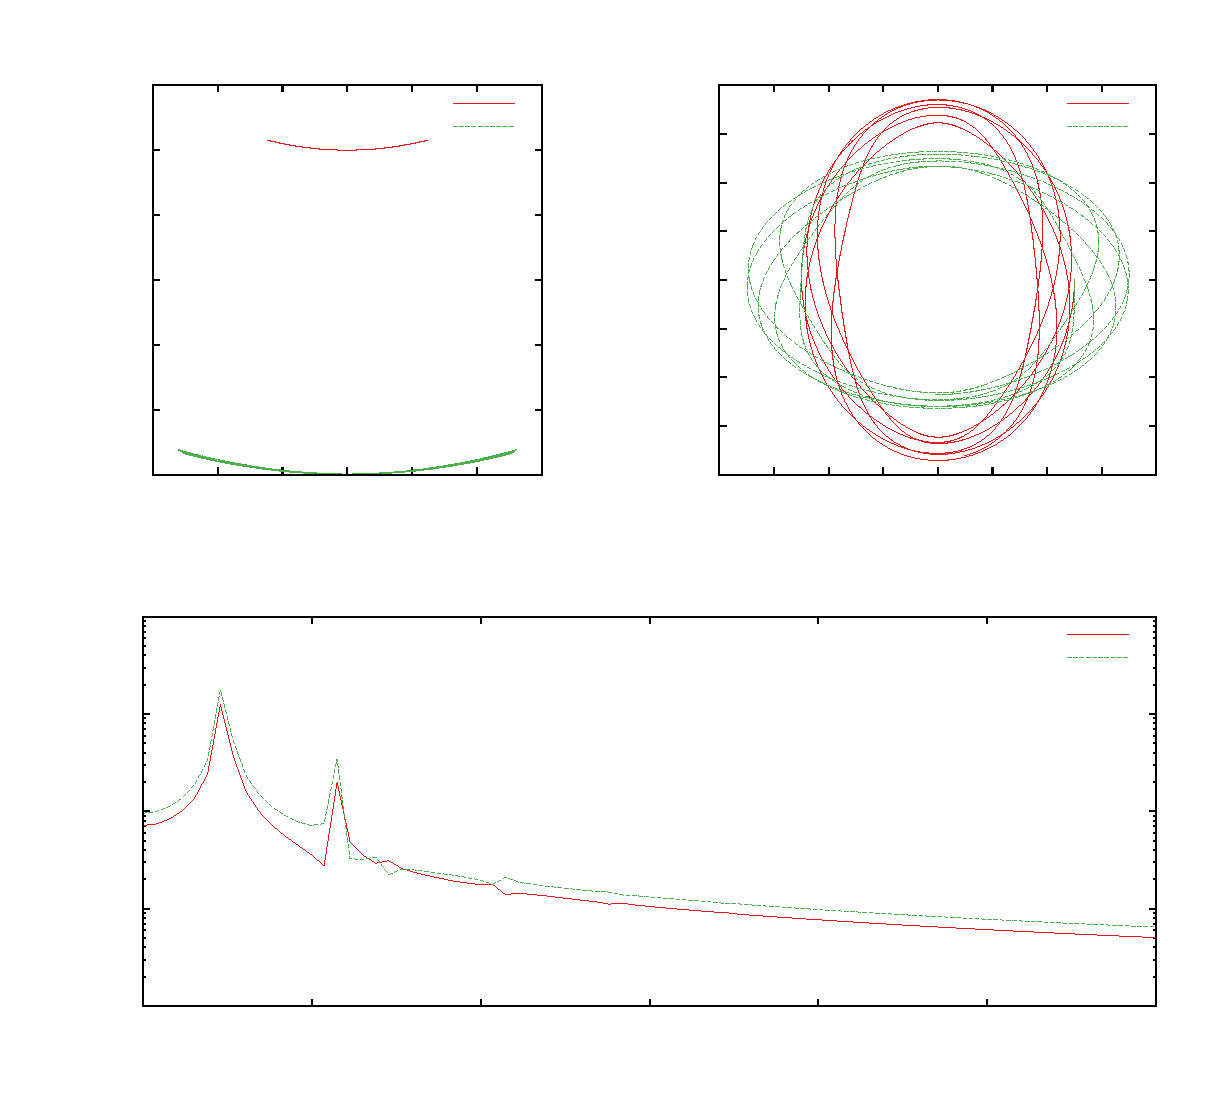
\includegraphics{./figures/trajektorie1}}%
    \gplfronttext
  \end{picture}%
\endgroup
}
\caption{Doppelpendel über einen Zeitraum von $t = \num{16.4} \, \si{\second}$ in Schritten von $h = \num{0.001} \, \si{\second}$. Anfangsbedingung: $\theta_1 = \theta_2 = \num{0.25}$, $\omega_1 = \omega_2 = \num{0} \, \si{\per\second}$.}
\label{fig1}
\end{figure}

\begin{figure}[htbp]
\centering
\scalebox{0.85}{% GNUPLOT: LaTeX picture with Postscript
\begingroup
  \makeatletter
  \providecommand\color[2][]{%
    \GenericError{(gnuplot) \space\space\space\@spaces}{%
      Package color not loaded in conjunction with
      terminal option `colourtext'%
    }{See the gnuplot documentation for explanation.%
    }{Either use 'blacktext' in gnuplot or load the package
      color.sty in LaTeX.}%
    \renewcommand\color[2][]{}%
  }%
  \providecommand\includegraphics[2][]{%
    \GenericError{(gnuplot) \space\space\space\@spaces}{%
      Package graphicx or graphics not loaded%
    }{See the gnuplot documentation for explanation.%
    }{The gnuplot epslatex terminal needs graphicx.sty or graphics.sty.}%
    \renewcommand\includegraphics[2][]{}%
  }%
  \providecommand\rotatebox[2]{#2}%
  \@ifundefined{ifGPcolor}{%
    \newif\ifGPcolor
    \GPcolortrue
  }{}%
  \@ifundefined{ifGPblacktext}{%
    \newif\ifGPblacktext
    \GPblacktextfalse
  }{}%
  % define a \g@addto@macro without @ in the name:
  \let\gplgaddtomacro\g@addto@macro
  % define empty templates for all commands taking text:
  \gdef\gplbacktext{}%
  \gdef\gplfronttext{}%
  \makeatother
  \ifGPblacktext
    % no textcolor at all
    \def\colorrgb#1{}%
    \def\colorgray#1{}%
  \else
    % gray or color?
    \ifGPcolor
      \def\colorrgb#1{\color[rgb]{#1}}%
      \def\colorgray#1{\color[gray]{#1}}%
      \expandafter\def\csname LTw\endcsname{\color{white}}%
      \expandafter\def\csname LTb\endcsname{\color{black}}%
      \expandafter\def\csname LTa\endcsname{\color{black}}%
      \expandafter\def\csname LT0\endcsname{\color[rgb]{1,0,0}}%
      \expandafter\def\csname LT1\endcsname{\color[rgb]{0,1,0}}%
      \expandafter\def\csname LT2\endcsname{\color[rgb]{0,0,1}}%
      \expandafter\def\csname LT3\endcsname{\color[rgb]{1,0,1}}%
      \expandafter\def\csname LT4\endcsname{\color[rgb]{0,1,1}}%
      \expandafter\def\csname LT5\endcsname{\color[rgb]{1,1,0}}%
      \expandafter\def\csname LT6\endcsname{\color[rgb]{0,0,0}}%
      \expandafter\def\csname LT7\endcsname{\color[rgb]{1,0.3,0}}%
      \expandafter\def\csname LT8\endcsname{\color[rgb]{0.5,0.5,0.5}}%
    \else
      % gray
      \def\colorrgb#1{\color{black}}%
      \def\colorgray#1{\color[gray]{#1}}%
      \expandafter\def\csname LTw\endcsname{\color{white}}%
      \expandafter\def\csname LTb\endcsname{\color{black}}%
      \expandafter\def\csname LTa\endcsname{\color{black}}%
      \expandafter\def\csname LT0\endcsname{\color{black}}%
      \expandafter\def\csname LT1\endcsname{\color{black}}%
      \expandafter\def\csname LT2\endcsname{\color{black}}%
      \expandafter\def\csname LT3\endcsname{\color{black}}%
      \expandafter\def\csname LT4\endcsname{\color{black}}%
      \expandafter\def\csname LT5\endcsname{\color{black}}%
      \expandafter\def\csname LT6\endcsname{\color{black}}%
      \expandafter\def\csname LT7\endcsname{\color{black}}%
      \expandafter\def\csname LT8\endcsname{\color{black}}%
    \fi
  \fi
  \setlength{\unitlength}{0.0500bp}%
  \begin{picture}(11338.00,10204.00)%
    \gplgaddtomacro\gplbacktext{%
      \csname LTb\endcsname%
      \put(946,6476){\makebox(0,0)[r]{\strut{}-2}}%
      \put(946,6716){\makebox(0,0)[r]{\strut{}-1.8}}%
      \put(946,6955){\makebox(0,0)[r]{\strut{}-1.6}}%
      \put(946,7195){\makebox(0,0)[r]{\strut{}-1.4}}%
      \put(946,7435){\makebox(0,0)[r]{\strut{}-1.2}}%
      \put(946,7675){\makebox(0,0)[r]{\strut{}-1}}%
      \put(946,7914){\makebox(0,0)[r]{\strut{}-0.8}}%
      \put(946,8154){\makebox(0,0)[r]{\strut{}-0.6}}%
      \put(946,8394){\makebox(0,0)[r]{\strut{}-0.4}}%
      \put(946,8633){\makebox(0,0)[r]{\strut{}-0.2}}%
      \put(946,8873){\makebox(0,0)[r]{\strut{} 0}}%
      \put(1078,6256){\makebox(0,0){\strut{}-2}}%
      \put(1677,6256){\makebox(0,0){\strut{}-1.5}}%
      \put(2276,6256){\makebox(0,0){\strut{}-1}}%
      \put(2875,6256){\makebox(0,0){\strut{}-0.5}}%
      \put(3475,6256){\makebox(0,0){\strut{} 0}}%
      \put(4074,6256){\makebox(0,0){\strut{} 0.5}}%
      \put(4673,6256){\makebox(0,0){\strut{} 1}}%
      \put(5272,6256){\makebox(0,0){\strut{} 1.5}}%
      \put(176,7674){\rotatebox{-270}{\makebox(0,0){\strut{}Position $y$ [$\si{\metre}$]}}}%
      \put(3175,5926){\makebox(0,0){\strut{}Position $x$ [$\si{\metre}$]}}%
      \put(3175,9203){\makebox(0,0){\strut{}Trajektorie}}%
    }%
    \gplgaddtomacro\gplfronttext{%
      \csname LTb\endcsname%
      \put(4285,8700){\makebox(0,0)[r]{\strut{}$m_1$}}%
      \csname LTb\endcsname%
      \put(4285,8480){\makebox(0,0)[r]{\strut{}$m_2$}}%
    }%
    \gplgaddtomacro\gplbacktext{%
      \csname LTb\endcsname%
      \put(6351,5806){\makebox(0,0)[r]{\strut{}-8}}%
      \put(6351,6273){\makebox(0,0)[r]{\strut{}-6}}%
      \put(6351,6740){\makebox(0,0)[r]{\strut{}-4}}%
      \put(6351,7207){\makebox(0,0)[r]{\strut{}-2}}%
      \put(6351,7675){\makebox(0,0)[r]{\strut{} 0}}%
      \put(6351,8142){\makebox(0,0)[r]{\strut{} 2}}%
      \put(6351,8609){\makebox(0,0)[r]{\strut{} 4}}%
      \put(6351,9076){\makebox(0,0)[r]{\strut{} 6}}%
      \put(6351,9543){\makebox(0,0)[r]{\strut{} 8}}%
      \put(6483,5586){\makebox(0,0){\strut{}-2.5}}%
      \put(6888,5586){\makebox(0,0){\strut{}-2}}%
      \put(7294,5586){\makebox(0,0){\strut{}-1.5}}%
      \put(7699,5586){\makebox(0,0){\strut{}-1}}%
      \put(8104,5586){\makebox(0,0){\strut{}-0.5}}%
      \put(8509,5586){\makebox(0,0){\strut{} 0}}%
      \put(8915,5586){\makebox(0,0){\strut{} 0.5}}%
      \put(9320,5586){\makebox(0,0){\strut{} 1}}%
      \put(9725,5586){\makebox(0,0){\strut{} 1.5}}%
      \put(10130,5586){\makebox(0,0){\strut{} 2}}%
      \put(10536,5586){\makebox(0,0){\strut{} 2.5}}%
      \put(10941,5586){\makebox(0,0){\strut{} 3}}%
      \put(5845,7674){\rotatebox{-270}{\makebox(0,0){\strut{}verallgemeinerter Impuls $p_{\theta}$ [$\si{\kilogram\metre\squared\per\second}$]}}}%
      \put(8712,5256){\makebox(0,0){\strut{}Auslenkung $\theta$ [$\si{\radian}$]}}%
      \put(8712,9873){\makebox(0,0){\strut{}Phasenraum}}%
    }%
    \gplgaddtomacro\gplfronttext{%
      \csname LTb\endcsname%
      \put(9954,9370){\makebox(0,0)[r]{\strut{}$\theta_1$}}%
      \csname LTb\endcsname%
      \put(9954,9150){\makebox(0,0)[r]{\strut{}$\theta_2$}}%
    }%
    \gplgaddtomacro\gplbacktext{%
      \csname LTb\endcsname%
      \put(1210,704){\makebox(0,0)[r]{\strut{} 0.001}}%
      \put(1210,1452){\makebox(0,0)[r]{\strut{} 0.01}}%
      \put(1210,2199){\makebox(0,0)[r]{\strut{} 0.1}}%
      \put(1210,2947){\makebox(0,0)[r]{\strut{} 1}}%
      \put(1210,3694){\makebox(0,0)[r]{\strut{} 10}}%
      \put(1210,4442){\makebox(0,0)[r]{\strut{} 100}}%
      \put(1342,484){\makebox(0,0){\strut{} 0}}%
      \put(2542,484){\makebox(0,0){\strut{} 10}}%
      \put(3742,484){\makebox(0,0){\strut{} 20}}%
      \put(4942,484){\makebox(0,0){\strut{} 30}}%
      \put(6142,484){\makebox(0,0){\strut{} 40}}%
      \put(7341,484){\makebox(0,0){\strut{} 50}}%
      \put(8541,484){\makebox(0,0){\strut{} 60}}%
      \put(9741,484){\makebox(0,0){\strut{} 70}}%
      \put(10941,484){\makebox(0,0){\strut{} 80}}%
      \put(176,2573){\rotatebox{-270}{\makebox(0,0){\strut{}Fourierkoeffizient $|g_k|$ [$\si{\radian}$]}}}%
      \put(6141,154){\makebox(0,0){\strut{}Kreisfrequenz $\omega$ [$\si{\radian\per\second}$]}}%
      \put(6141,4772){\makebox(0,0){\strut{}Leistungsspektrum von $\theta$}}%
    }%
    \gplgaddtomacro\gplfronttext{%
      \csname LTb\endcsname%
      \put(9954,4269){\makebox(0,0)[r]{\strut{}$\theta_1$}}%
      \csname LTb\endcsname%
      \put(9954,4049){\makebox(0,0)[r]{\strut{}$\theta_2$}}%
    }%
    \gplbacktext
    \put(0,0){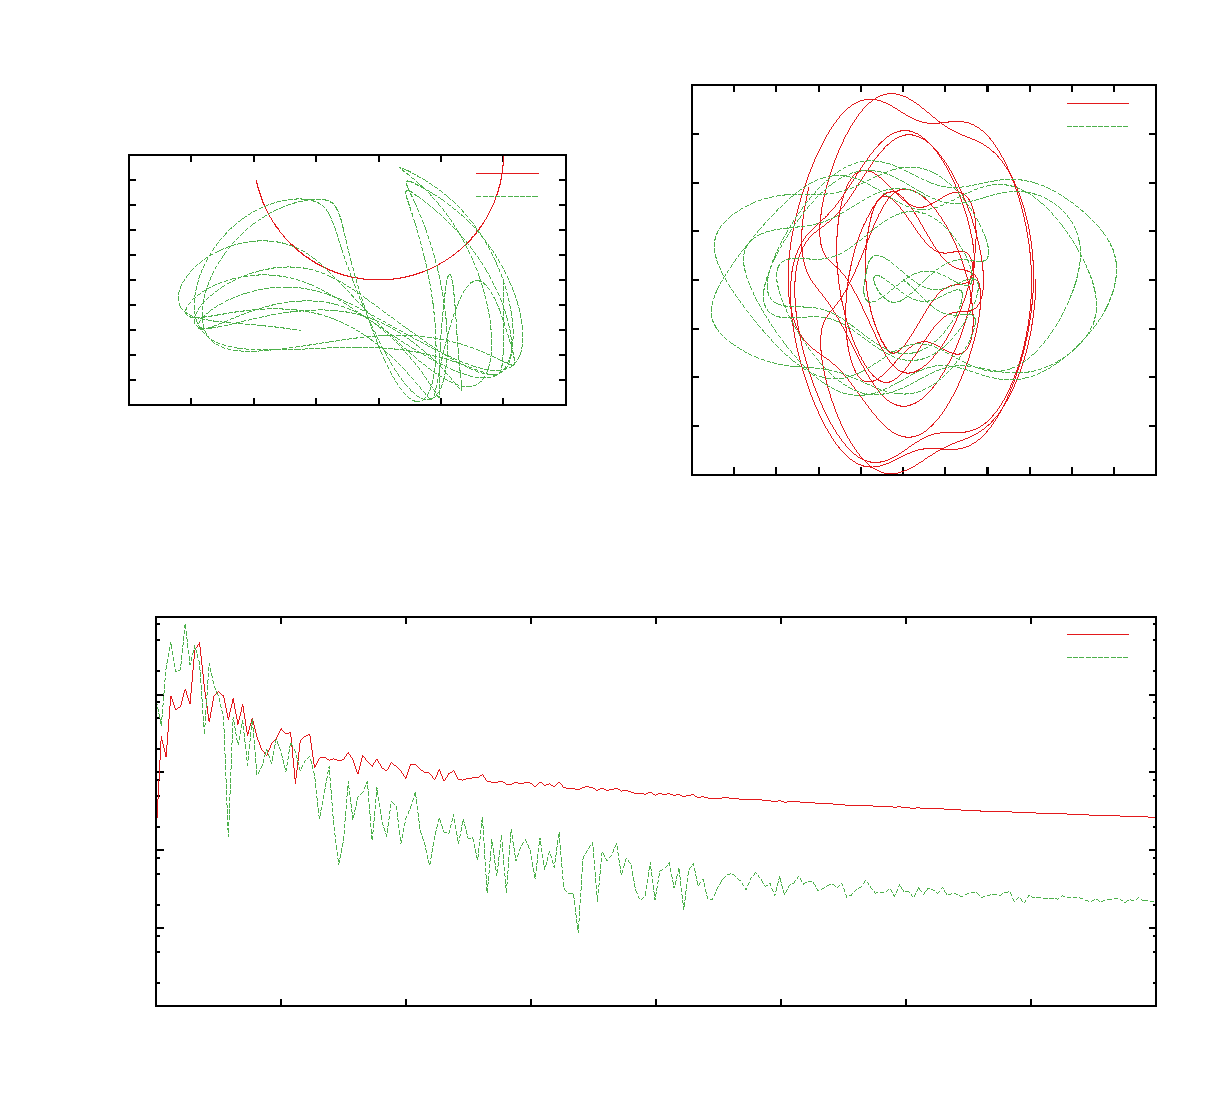
\includegraphics{./figures/trajektorie2}}%
    \gplfronttext
  \end{picture}%
\endgroup
}
\caption{Doppelpendel über einen Zeitraum von $t = \num{16.4} \, \si{\second}$ in Schritten von $h = \num{0.001} \, \si{\second}$. Anfangsbedingung: $\theta_1 = \frac{\pi}{2}$, $\theta_2 = \num{0}$, $\omega_1 = \omega_2 = \num{0} \, \si{\per\second}$.}
\label{fig2}
\end{figure}

\begin{figure}[htbp]
\centering
\scalebox{0.85}{% GNUPLOT: LaTeX picture with Postscript
\begingroup
  \makeatletter
  \providecommand\color[2][]{%
    \GenericError{(gnuplot) \space\space\space\@spaces}{%
      Package color not loaded in conjunction with
      terminal option `colourtext'%
    }{See the gnuplot documentation for explanation.%
    }{Either use 'blacktext' in gnuplot or load the package
      color.sty in LaTeX.}%
    \renewcommand\color[2][]{}%
  }%
  \providecommand\includegraphics[2][]{%
    \GenericError{(gnuplot) \space\space\space\@spaces}{%
      Package graphicx or graphics not loaded%
    }{See the gnuplot documentation for explanation.%
    }{The gnuplot epslatex terminal needs graphicx.sty or graphics.sty.}%
    \renewcommand\includegraphics[2][]{}%
  }%
  \providecommand\rotatebox[2]{#2}%
  \@ifundefined{ifGPcolor}{%
    \newif\ifGPcolor
    \GPcolortrue
  }{}%
  \@ifundefined{ifGPblacktext}{%
    \newif\ifGPblacktext
    \GPblacktextfalse
  }{}%
  % define a \g@addto@macro without @ in the name:
  \let\gplgaddtomacro\g@addto@macro
  % define empty templates for all commands taking text:
  \gdef\gplbacktext{}%
  \gdef\gplfronttext{}%
  \makeatother
  \ifGPblacktext
    % no textcolor at all
    \def\colorrgb#1{}%
    \def\colorgray#1{}%
  \else
    % gray or color?
    \ifGPcolor
      \def\colorrgb#1{\color[rgb]{#1}}%
      \def\colorgray#1{\color[gray]{#1}}%
      \expandafter\def\csname LTw\endcsname{\color{white}}%
      \expandafter\def\csname LTb\endcsname{\color{black}}%
      \expandafter\def\csname LTa\endcsname{\color{black}}%
      \expandafter\def\csname LT0\endcsname{\color[rgb]{1,0,0}}%
      \expandafter\def\csname LT1\endcsname{\color[rgb]{0,1,0}}%
      \expandafter\def\csname LT2\endcsname{\color[rgb]{0,0,1}}%
      \expandafter\def\csname LT3\endcsname{\color[rgb]{1,0,1}}%
      \expandafter\def\csname LT4\endcsname{\color[rgb]{0,1,1}}%
      \expandafter\def\csname LT5\endcsname{\color[rgb]{1,1,0}}%
      \expandafter\def\csname LT6\endcsname{\color[rgb]{0,0,0}}%
      \expandafter\def\csname LT7\endcsname{\color[rgb]{1,0.3,0}}%
      \expandafter\def\csname LT8\endcsname{\color[rgb]{0.5,0.5,0.5}}%
    \else
      % gray
      \def\colorrgb#1{\color{black}}%
      \def\colorgray#1{\color[gray]{#1}}%
      \expandafter\def\csname LTw\endcsname{\color{white}}%
      \expandafter\def\csname LTb\endcsname{\color{black}}%
      \expandafter\def\csname LTa\endcsname{\color{black}}%
      \expandafter\def\csname LT0\endcsname{\color{black}}%
      \expandafter\def\csname LT1\endcsname{\color{black}}%
      \expandafter\def\csname LT2\endcsname{\color{black}}%
      \expandafter\def\csname LT3\endcsname{\color{black}}%
      \expandafter\def\csname LT4\endcsname{\color{black}}%
      \expandafter\def\csname LT5\endcsname{\color{black}}%
      \expandafter\def\csname LT6\endcsname{\color{black}}%
      \expandafter\def\csname LT7\endcsname{\color{black}}%
      \expandafter\def\csname LT8\endcsname{\color{black}}%
    \fi
  \fi
  \setlength{\unitlength}{0.0500bp}%
  \begin{picture}(11338.00,10204.00)%
    \gplgaddtomacro\gplbacktext{%
      \csname LTb\endcsname%
      \put(1174,5806){\makebox(0,0)[r]{\strut{}-2}}%
      \put(1174,6273){\makebox(0,0)[r]{\strut{}-1.5}}%
      \put(1174,6740){\makebox(0,0)[r]{\strut{}-1}}%
      \put(1174,7207){\makebox(0,0)[r]{\strut{}-0.5}}%
      \put(1174,7675){\makebox(0,0)[r]{\strut{} 0}}%
      \put(1174,8142){\makebox(0,0)[r]{\strut{} 0.5}}%
      \put(1174,8609){\makebox(0,0)[r]{\strut{} 1}}%
      \put(1174,9076){\makebox(0,0)[r]{\strut{} 1.5}}%
      \put(1174,9543){\makebox(0,0)[r]{\strut{} 2}}%
      \put(1306,5586){\makebox(0,0){\strut{}-2}}%
      \put(1773,5586){\makebox(0,0){\strut{}-1.5}}%
      \put(2241,5586){\makebox(0,0){\strut{}-1}}%
      \put(2708,5586){\makebox(0,0){\strut{}-0.5}}%
      \put(3175,5586){\makebox(0,0){\strut{} 0}}%
      \put(3642,5586){\makebox(0,0){\strut{} 0.5}}%
      \put(4110,5586){\makebox(0,0){\strut{} 1}}%
      \put(4577,5586){\makebox(0,0){\strut{} 1.5}}%
      \put(5044,5586){\makebox(0,0){\strut{} 2}}%
      \put(404,7674){\rotatebox{-270}{\makebox(0,0){\strut{}Position $y$ [$\si{\metre}$]}}}%
      \put(3175,5256){\makebox(0,0){\strut{}Position $x$ [$\si{\metre}$]}}%
      \put(3175,9873){\makebox(0,0){\strut{}Trajektorie}}%
    }%
    \gplgaddtomacro\gplfronttext{%
      \csname LTb\endcsname%
      \put(4057,9370){\makebox(0,0)[r]{\strut{}$m_1$}}%
      \csname LTb\endcsname%
      \put(4057,9150){\makebox(0,0)[r]{\strut{}$m_2$}}%
    }%
    \gplgaddtomacro\gplbacktext{%
      \csname LTb\endcsname%
      \put(6483,5806){\makebox(0,0)[r]{\strut{}-15}}%
      \put(6483,6429){\makebox(0,0)[r]{\strut{}-10}}%
      \put(6483,7052){\makebox(0,0)[r]{\strut{}-5}}%
      \put(6483,7675){\makebox(0,0)[r]{\strut{} 0}}%
      \put(6483,8297){\makebox(0,0)[r]{\strut{} 5}}%
      \put(6483,8920){\makebox(0,0)[r]{\strut{} 10}}%
      \put(6483,9543){\makebox(0,0)[r]{\strut{} 15}}%
      \put(6615,5586){\makebox(0,0){\strut{}-10}}%
      \put(7008,5586){\makebox(0,0){\strut{}-5}}%
      \put(7402,5586){\makebox(0,0){\strut{} 0}}%
      \put(7795,5586){\makebox(0,0){\strut{} 5}}%
      \put(8188,5586){\makebox(0,0){\strut{} 10}}%
      \put(8581,5586){\makebox(0,0){\strut{} 15}}%
      \put(8975,5586){\makebox(0,0){\strut{} 20}}%
      \put(9368,5586){\makebox(0,0){\strut{} 25}}%
      \put(9761,5586){\makebox(0,0){\strut{} 30}}%
      \put(10154,5586){\makebox(0,0){\strut{} 35}}%
      \put(10548,5586){\makebox(0,0){\strut{} 40}}%
      \put(10941,5586){\makebox(0,0){\strut{} 45}}%
      \put(5845,7674){\rotatebox{-270}{\makebox(0,0){\strut{}verallgemeinerter Impuls $p_{\theta}$ [$\si{\kilogram\metre\squared\per\second}$]}}}%
      \put(8778,5256){\makebox(0,0){\strut{}Auslenkung $\theta$ [$\si{\radian}$]}}%
      \put(8778,9873){\makebox(0,0){\strut{}Phasenraum}}%
    }%
    \gplgaddtomacro\gplfronttext{%
      \csname LTb\endcsname%
      \put(9954,9370){\makebox(0,0)[r]{\strut{}$\theta_1$}}%
      \csname LTb\endcsname%
      \put(9954,9150){\makebox(0,0)[r]{\strut{}$\theta_2$}}%
    }%
    \gplgaddtomacro\gplbacktext{%
      \csname LTb\endcsname%
      \put(1210,704){\makebox(0,0)[r]{\strut{} 1}}%
      \put(1210,1639){\makebox(0,0)[r]{\strut{} 10}}%
      \put(1210,2573){\makebox(0,0)[r]{\strut{} 100}}%
      \put(1210,3508){\makebox(0,0)[r]{\strut{} 1000}}%
      \put(1210,4442){\makebox(0,0)[r]{\strut{} 10000}}%
      \put(1342,484){\makebox(0,0){\strut{} 0}}%
      \put(2542,484){\makebox(0,0){\strut{} 10}}%
      \put(3742,484){\makebox(0,0){\strut{} 20}}%
      \put(4942,484){\makebox(0,0){\strut{} 30}}%
      \put(6142,484){\makebox(0,0){\strut{} 40}}%
      \put(7341,484){\makebox(0,0){\strut{} 50}}%
      \put(8541,484){\makebox(0,0){\strut{} 60}}%
      \put(9741,484){\makebox(0,0){\strut{} 70}}%
      \put(10941,484){\makebox(0,0){\strut{} 80}}%
      \put(176,2573){\rotatebox{-270}{\makebox(0,0){\strut{}Fourierkoeffizient $|g_k|$ [$\si{\radian}$]}}}%
      \put(6141,154){\makebox(0,0){\strut{}Kreisfrequenz $\omega$ [$\si{\radian\per\second}$]}}%
      \put(6141,4772){\makebox(0,0){\strut{}Leistungsspektrum von $\theta$}}%
    }%
    \gplgaddtomacro\gplfronttext{%
      \csname LTb\endcsname%
      \put(9954,4269){\makebox(0,0)[r]{\strut{}$\theta_1$}}%
      \csname LTb\endcsname%
      \put(9954,4049){\makebox(0,0)[r]{\strut{}$\theta_2$}}%
    }%
    \gplbacktext
    \put(0,0){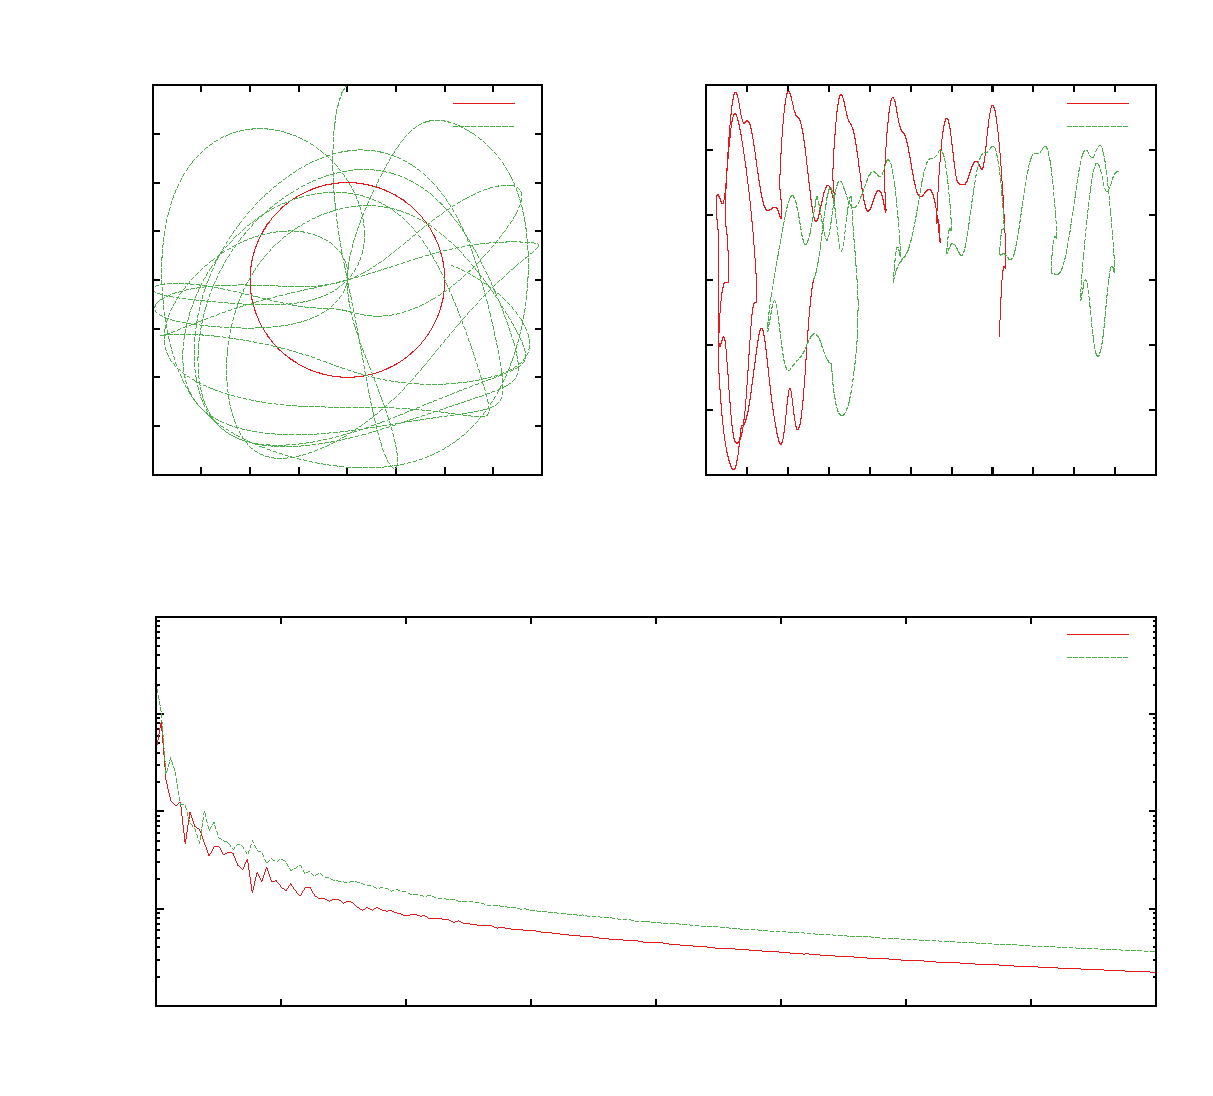
\includegraphics{./figures/trajektorie3}}%
    \gplfronttext
  \end{picture}%
\endgroup
}
\caption{Doppelpendel über einen Zeitraum von $t = \num{16.4} \, \si{\second}$ in Schritten von $h = \num{0.001} \, \si{\second}$. Anfangsbedingung: $\theta_1 = \theta_2 = \num{3.14}$, $\omega_1 = \omega_2 = \num{0} \, \si{\per\second}$.}
\label{fig3}
\end{figure}

\begin{figure}[htbp]
\centering
\scalebox{0.85}{% GNUPLOT: LaTeX picture with Postscript
\begingroup
  \makeatletter
  \providecommand\color[2][]{%
    \GenericError{(gnuplot) \space\space\space\@spaces}{%
      Package color not loaded in conjunction with
      terminal option `colourtext'%
    }{See the gnuplot documentation for explanation.%
    }{Either use 'blacktext' in gnuplot or load the package
      color.sty in LaTeX.}%
    \renewcommand\color[2][]{}%
  }%
  \providecommand\includegraphics[2][]{%
    \GenericError{(gnuplot) \space\space\space\@spaces}{%
      Package graphicx or graphics not loaded%
    }{See the gnuplot documentation for explanation.%
    }{The gnuplot epslatex terminal needs graphicx.sty or graphics.sty.}%
    \renewcommand\includegraphics[2][]{}%
  }%
  \providecommand\rotatebox[2]{#2}%
  \@ifundefined{ifGPcolor}{%
    \newif\ifGPcolor
    \GPcolortrue
  }{}%
  \@ifundefined{ifGPblacktext}{%
    \newif\ifGPblacktext
    \GPblacktextfalse
  }{}%
  % define a \g@addto@macro without @ in the name:
  \let\gplgaddtomacro\g@addto@macro
  % define empty templates for all commands taking text:
  \gdef\gplbacktext{}%
  \gdef\gplfronttext{}%
  \makeatother
  \ifGPblacktext
    % no textcolor at all
    \def\colorrgb#1{}%
    \def\colorgray#1{}%
  \else
    % gray or color?
    \ifGPcolor
      \def\colorrgb#1{\color[rgb]{#1}}%
      \def\colorgray#1{\color[gray]{#1}}%
      \expandafter\def\csname LTw\endcsname{\color{white}}%
      \expandafter\def\csname LTb\endcsname{\color{black}}%
      \expandafter\def\csname LTa\endcsname{\color{black}}%
      \expandafter\def\csname LT0\endcsname{\color[rgb]{1,0,0}}%
      \expandafter\def\csname LT1\endcsname{\color[rgb]{0,1,0}}%
      \expandafter\def\csname LT2\endcsname{\color[rgb]{0,0,1}}%
      \expandafter\def\csname LT3\endcsname{\color[rgb]{1,0,1}}%
      \expandafter\def\csname LT4\endcsname{\color[rgb]{0,1,1}}%
      \expandafter\def\csname LT5\endcsname{\color[rgb]{1,1,0}}%
      \expandafter\def\csname LT6\endcsname{\color[rgb]{0,0,0}}%
      \expandafter\def\csname LT7\endcsname{\color[rgb]{1,0.3,0}}%
      \expandafter\def\csname LT8\endcsname{\color[rgb]{0.5,0.5,0.5}}%
    \else
      % gray
      \def\colorrgb#1{\color{black}}%
      \def\colorgray#1{\color[gray]{#1}}%
      \expandafter\def\csname LTw\endcsname{\color{white}}%
      \expandafter\def\csname LTb\endcsname{\color{black}}%
      \expandafter\def\csname LTa\endcsname{\color{black}}%
      \expandafter\def\csname LT0\endcsname{\color{black}}%
      \expandafter\def\csname LT1\endcsname{\color{black}}%
      \expandafter\def\csname LT2\endcsname{\color{black}}%
      \expandafter\def\csname LT3\endcsname{\color{black}}%
      \expandafter\def\csname LT4\endcsname{\color{black}}%
      \expandafter\def\csname LT5\endcsname{\color{black}}%
      \expandafter\def\csname LT6\endcsname{\color{black}}%
      \expandafter\def\csname LT7\endcsname{\color{black}}%
      \expandafter\def\csname LT8\endcsname{\color{black}}%
    \fi
  \fi
  \setlength{\unitlength}{0.0500bp}%
  \begin{picture}(11338.00,10204.00)%
    \gplgaddtomacro\gplbacktext{%
      \csname LTb\endcsname%
      \put(946,6696){\makebox(0,0)[r]{\strut{}-2}}%
      \put(946,6976){\makebox(0,0)[r]{\strut{}-1.8}}%
      \put(946,7255){\makebox(0,0)[r]{\strut{}-1.6}}%
      \put(946,7535){\makebox(0,0)[r]{\strut{}-1.4}}%
      \put(946,7814){\makebox(0,0)[r]{\strut{}-1.2}}%
      \put(946,8094){\makebox(0,0)[r]{\strut{}-1}}%
      \put(946,8373){\makebox(0,0)[r]{\strut{}-0.8}}%
      \put(946,8653){\makebox(0,0)[r]{\strut{}-0.6}}%
      \put(1078,6476){\makebox(0,0){\strut{}-1.5}}%
      \put(1777,6476){\makebox(0,0){\strut{}-1}}%
      \put(2476,6476){\makebox(0,0){\strut{}-0.5}}%
      \put(3175,6476){\makebox(0,0){\strut{} 0}}%
      \put(3874,6476){\makebox(0,0){\strut{} 0.5}}%
      \put(4573,6476){\makebox(0,0){\strut{} 1}}%
      \put(5272,6476){\makebox(0,0){\strut{} 1.5}}%
      \put(176,7674){\rotatebox{-270}{\makebox(0,0){\strut{}Position $y$ [$\si{\metre}$]}}}%
      \put(3175,6146){\makebox(0,0){\strut{}Position $x$ [$\si{\metre}$]}}%
      \put(3175,8983){\makebox(0,0){\strut{}Trajektorie}}%
    }%
    \gplgaddtomacro\gplfronttext{%
      \csname LTb\endcsname%
      \put(4285,8480){\makebox(0,0)[r]{\strut{}$m_1$}}%
      \csname LTb\endcsname%
      \put(4285,8260){\makebox(0,0)[r]{\strut{}$m_2$}}%
    }%
    \gplgaddtomacro\gplbacktext{%
      \csname LTb\endcsname%
      \put(6351,5806){\makebox(0,0)[r]{\strut{}-6}}%
      \put(6351,6429){\makebox(0,0)[r]{\strut{}-4}}%
      \put(6351,7052){\makebox(0,0)[r]{\strut{}-2}}%
      \put(6351,7675){\makebox(0,0)[r]{\strut{} 0}}%
      \put(6351,8297){\makebox(0,0)[r]{\strut{} 2}}%
      \put(6351,8920){\makebox(0,0)[r]{\strut{} 4}}%
      \put(6351,9543){\makebox(0,0)[r]{\strut{} 6}}%
      \put(6483,5586){\makebox(0,0){\strut{}-1.5}}%
      \put(7226,5586){\makebox(0,0){\strut{}-1}}%
      \put(7969,5586){\makebox(0,0){\strut{}-0.5}}%
      \put(8712,5586){\makebox(0,0){\strut{} 0}}%
      \put(9455,5586){\makebox(0,0){\strut{} 0.5}}%
      \put(10198,5586){\makebox(0,0){\strut{} 1}}%
      \put(10941,5586){\makebox(0,0){\strut{} 1.5}}%
      \put(5845,7674){\rotatebox{-270}{\makebox(0,0){\strut{}verallgemeinerter Impuls $p_{\theta}$ [$\si{\kilogram\metre\squared\per\second}$]}}}%
      \put(8712,5256){\makebox(0,0){\strut{}Auslenkung $\theta$ [$\si{\radian}$]}}%
      \put(8712,9873){\makebox(0,0){\strut{}Phasenraum}}%
    }%
    \gplgaddtomacro\gplfronttext{%
      \csname LTb\endcsname%
      \put(9954,9370){\makebox(0,0)[r]{\strut{}$\theta_1$}}%
      \csname LTb\endcsname%
      \put(9954,9150){\makebox(0,0)[r]{\strut{}$\theta_2$}}%
    }%
    \gplgaddtomacro\gplbacktext{%
      \csname LTb\endcsname%
      \put(1078,704){\makebox(0,0)[r]{\strut{} 0.01}}%
      \put(1078,1639){\makebox(0,0)[r]{\strut{} 0.1}}%
      \put(1078,2573){\makebox(0,0)[r]{\strut{} 1}}%
      \put(1078,3508){\makebox(0,0)[r]{\strut{} 10}}%
      \put(1078,4442){\makebox(0,0)[r]{\strut{} 100}}%
      \put(1210,484){\makebox(0,0){\strut{} 0}}%
      \put(2426,484){\makebox(0,0){\strut{} 5}}%
      \put(3643,484){\makebox(0,0){\strut{} 10}}%
      \put(4859,484){\makebox(0,0){\strut{} 15}}%
      \put(6076,484){\makebox(0,0){\strut{} 20}}%
      \put(7292,484){\makebox(0,0){\strut{} 25}}%
      \put(8508,484){\makebox(0,0){\strut{} 30}}%
      \put(9725,484){\makebox(0,0){\strut{} 35}}%
      \put(10941,484){\makebox(0,0){\strut{} 40}}%
      \put(176,2573){\rotatebox{-270}{\makebox(0,0){\strut{}Fourierkoeffizient $|g_k|$ [$\si{\radian}$]}}}%
      \put(6075,154){\makebox(0,0){\strut{}Kreisfrequenz $\omega$ [$\si{\radian\per\second}$]}}%
      \put(6075,4772){\makebox(0,0){\strut{}Leistungsspektrum von $\theta$}}%
    }%
    \gplgaddtomacro\gplfronttext{%
      \csname LTb\endcsname%
      \put(9954,4269){\makebox(0,0)[r]{\strut{}$\theta_1$}}%
      \csname LTb\endcsname%
      \put(9954,4049){\makebox(0,0)[r]{\strut{}$\theta_2$}}%
    }%
    \gplbacktext
    \put(0,0){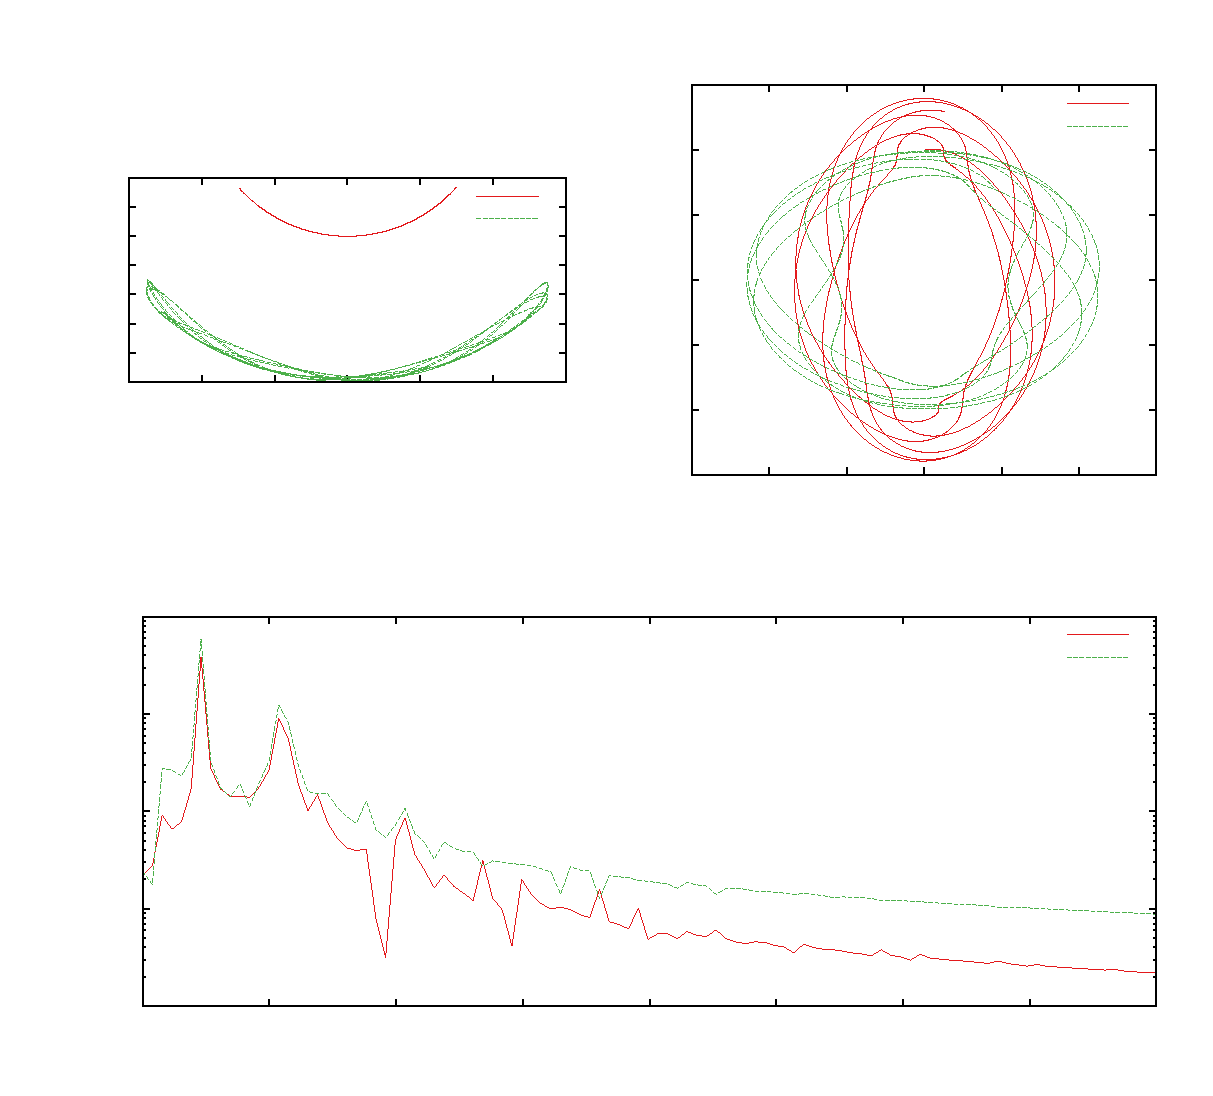
\includegraphics{./figures/trajektorie4}}%
    \gplfronttext
  \end{picture}%
\endgroup
}
\caption{Doppelpendel über einen Zeitraum von $t = \num{16.4} \, \si{\second}$ in Schritten von $h = \num{0.001} \, \si{\second}$. Anfangsbedingung: $\theta_1 = \theta_2 = \num{0}$, $\omega_1 = \num{0} \, \si{\per\second}$, $\omega_2 = \num{4} \, \si{\per\second}$.}
\label{fig4}
\end{figure}

\begin{figure}[htbp]
\centering
\scalebox{0.85}{% GNUPLOT: LaTeX picture with Postscript
\begingroup
  \makeatletter
  \providecommand\color[2][]{%
    \GenericError{(gnuplot) \space\space\space\@spaces}{%
      Package color not loaded in conjunction with
      terminal option `colourtext'%
    }{See the gnuplot documentation for explanation.%
    }{Either use 'blacktext' in gnuplot or load the package
      color.sty in LaTeX.}%
    \renewcommand\color[2][]{}%
  }%
  \providecommand\includegraphics[2][]{%
    \GenericError{(gnuplot) \space\space\space\@spaces}{%
      Package graphicx or graphics not loaded%
    }{See the gnuplot documentation for explanation.%
    }{The gnuplot epslatex terminal needs graphicx.sty or graphics.sty.}%
    \renewcommand\includegraphics[2][]{}%
  }%
  \providecommand\rotatebox[2]{#2}%
  \@ifundefined{ifGPcolor}{%
    \newif\ifGPcolor
    \GPcolortrue
  }{}%
  \@ifundefined{ifGPblacktext}{%
    \newif\ifGPblacktext
    \GPblacktextfalse
  }{}%
  % define a \g@addto@macro without @ in the name:
  \let\gplgaddtomacro\g@addto@macro
  % define empty templates for all commands taking text:
  \gdef\gplbacktext{}%
  \gdef\gplfronttext{}%
  \makeatother
  \ifGPblacktext
    % no textcolor at all
    \def\colorrgb#1{}%
    \def\colorgray#1{}%
  \else
    % gray or color?
    \ifGPcolor
      \def\colorrgb#1{\color[rgb]{#1}}%
      \def\colorgray#1{\color[gray]{#1}}%
      \expandafter\def\csname LTw\endcsname{\color{white}}%
      \expandafter\def\csname LTb\endcsname{\color{black}}%
      \expandafter\def\csname LTa\endcsname{\color{black}}%
      \expandafter\def\csname LT0\endcsname{\color[rgb]{1,0,0}}%
      \expandafter\def\csname LT1\endcsname{\color[rgb]{0,1,0}}%
      \expandafter\def\csname LT2\endcsname{\color[rgb]{0,0,1}}%
      \expandafter\def\csname LT3\endcsname{\color[rgb]{1,0,1}}%
      \expandafter\def\csname LT4\endcsname{\color[rgb]{0,1,1}}%
      \expandafter\def\csname LT5\endcsname{\color[rgb]{1,1,0}}%
      \expandafter\def\csname LT6\endcsname{\color[rgb]{0,0,0}}%
      \expandafter\def\csname LT7\endcsname{\color[rgb]{1,0.3,0}}%
      \expandafter\def\csname LT8\endcsname{\color[rgb]{0.5,0.5,0.5}}%
    \else
      % gray
      \def\colorrgb#1{\color{black}}%
      \def\colorgray#1{\color[gray]{#1}}%
      \expandafter\def\csname LTw\endcsname{\color{white}}%
      \expandafter\def\csname LTb\endcsname{\color{black}}%
      \expandafter\def\csname LTa\endcsname{\color{black}}%
      \expandafter\def\csname LT0\endcsname{\color{black}}%
      \expandafter\def\csname LT1\endcsname{\color{black}}%
      \expandafter\def\csname LT2\endcsname{\color{black}}%
      \expandafter\def\csname LT3\endcsname{\color{black}}%
      \expandafter\def\csname LT4\endcsname{\color{black}}%
      \expandafter\def\csname LT5\endcsname{\color{black}}%
      \expandafter\def\csname LT6\endcsname{\color{black}}%
      \expandafter\def\csname LT7\endcsname{\color{black}}%
      \expandafter\def\csname LT8\endcsname{\color{black}}%
    \fi
  \fi
  \setlength{\unitlength}{0.0500bp}%
  \begin{picture}(11338.00,10204.00)%
    \gplgaddtomacro\gplbacktext{%
      \csname LTb\endcsname%
      \put(946,5840){\makebox(0,0)[r]{\strut{}-2}}%
      \put(946,6364){\makebox(0,0)[r]{\strut{}-1.8}}%
      \put(946,6888){\makebox(0,0)[r]{\strut{}-1.6}}%
      \put(946,7412){\makebox(0,0)[r]{\strut{}-1.4}}%
      \put(946,7937){\makebox(0,0)[r]{\strut{}-1.2}}%
      \put(946,8461){\makebox(0,0)[r]{\strut{}-1}}%
      \put(946,8985){\makebox(0,0)[r]{\strut{}-0.8}}%
      \put(946,9509){\makebox(0,0)[r]{\strut{}-0.6}}%
      \put(1078,5620){\makebox(0,0){\strut{}-0.8}}%
      \put(1602,5620){\makebox(0,0){\strut{}-0.6}}%
      \put(2127,5620){\makebox(0,0){\strut{}-0.4}}%
      \put(2651,5620){\makebox(0,0){\strut{}-0.2}}%
      \put(3175,5620){\makebox(0,0){\strut{} 0}}%
      \put(3699,5620){\makebox(0,0){\strut{} 0.2}}%
      \put(4224,5620){\makebox(0,0){\strut{} 0.4}}%
      \put(4748,5620){\makebox(0,0){\strut{} 0.6}}%
      \put(5272,5620){\makebox(0,0){\strut{} 0.8}}%
      \put(176,7674){\rotatebox{-270}{\makebox(0,0){\strut{}Position $y$ [$\si{\metre}$]}}}%
      \put(3175,5290){\makebox(0,0){\strut{}Position $x$ [$\si{\metre}$]}}%
      \put(3175,9839){\makebox(0,0){\strut{}Trajektorie}}%
    }%
    \gplgaddtomacro\gplfronttext{%
      \csname LTb\endcsname%
      \put(4285,9336){\makebox(0,0)[r]{\strut{}$m_1$}}%
      \csname LTb\endcsname%
      \put(4285,9116){\makebox(0,0)[r]{\strut{}$m_2$}}%
    }%
    \gplgaddtomacro\gplbacktext{%
      \csname LTb\endcsname%
      \put(6351,5806){\makebox(0,0)[r]{\strut{}-4}}%
      \put(6351,6273){\makebox(0,0)[r]{\strut{}-3}}%
      \put(6351,6740){\makebox(0,0)[r]{\strut{}-2}}%
      \put(6351,7207){\makebox(0,0)[r]{\strut{}-1}}%
      \put(6351,7675){\makebox(0,0)[r]{\strut{} 0}}%
      \put(6351,8142){\makebox(0,0)[r]{\strut{} 1}}%
      \put(6351,8609){\makebox(0,0)[r]{\strut{} 2}}%
      \put(6351,9076){\makebox(0,0)[r]{\strut{} 3}}%
      \put(6351,9543){\makebox(0,0)[r]{\strut{} 4}}%
      \put(6483,5586){\makebox(0,0){\strut{}-1.5}}%
      \put(7226,5586){\makebox(0,0){\strut{}-1}}%
      \put(7969,5586){\makebox(0,0){\strut{}-0.5}}%
      \put(8712,5586){\makebox(0,0){\strut{} 0}}%
      \put(9455,5586){\makebox(0,0){\strut{} 0.5}}%
      \put(10198,5586){\makebox(0,0){\strut{} 1}}%
      \put(10941,5586){\makebox(0,0){\strut{} 1.5}}%
      \put(5845,7674){\rotatebox{-270}{\makebox(0,0){\strut{}verallgemeinerter Impuls $p_{\theta}$ [$\si{\kilogram\metre\squared\per\second}$]}}}%
      \put(8712,5256){\makebox(0,0){\strut{}Auslenkung $\theta$ [$\si{\radian}$]}}%
      \put(8712,9873){\makebox(0,0){\strut{}Phasenraum}}%
    }%
    \gplgaddtomacro\gplfronttext{%
      \csname LTb\endcsname%
      \put(9954,9370){\makebox(0,0)[r]{\strut{}$\theta_1$}}%
      \csname LTb\endcsname%
      \put(9954,9150){\makebox(0,0)[r]{\strut{}$\theta_2$}}%
    }%
    \gplgaddtomacro\gplbacktext{%
      \csname LTb\endcsname%
      \put(946,704){\makebox(0,0)[r]{\strut{} 0.1}}%
      \put(946,1950){\makebox(0,0)[r]{\strut{} 1}}%
      \put(946,3196){\makebox(0,0)[r]{\strut{} 10}}%
      \put(946,4442){\makebox(0,0)[r]{\strut{} 100}}%
      \put(1078,484){\makebox(0,0){\strut{} 0}}%
      \put(2311,484){\makebox(0,0){\strut{} 5}}%
      \put(3544,484){\makebox(0,0){\strut{} 10}}%
      \put(4777,484){\makebox(0,0){\strut{} 15}}%
      \put(6010,484){\makebox(0,0){\strut{} 20}}%
      \put(7242,484){\makebox(0,0){\strut{} 25}}%
      \put(8475,484){\makebox(0,0){\strut{} 30}}%
      \put(9708,484){\makebox(0,0){\strut{} 35}}%
      \put(10941,484){\makebox(0,0){\strut{} 40}}%
      \put(176,2573){\rotatebox{-270}{\makebox(0,0){\strut{}Fourierkoeffizient $|g_k|$ [$\si{\radian}$]}}}%
      \put(6009,154){\makebox(0,0){\strut{}Kreisfrequenz $\omega$ [$\si{\radian\per\second}$]}}%
      \put(6009,4772){\makebox(0,0){\strut{}Leistungsspektrum von $\theta$}}%
    }%
    \gplgaddtomacro\gplfronttext{%
      \csname LTb\endcsname%
      \put(9954,4269){\makebox(0,0)[r]{\strut{}$\theta_1$}}%
      \csname LTb\endcsname%
      \put(9954,4049){\makebox(0,0)[r]{\strut{}$\theta_2$}}%
    }%
    \gplbacktext
    \put(0,0){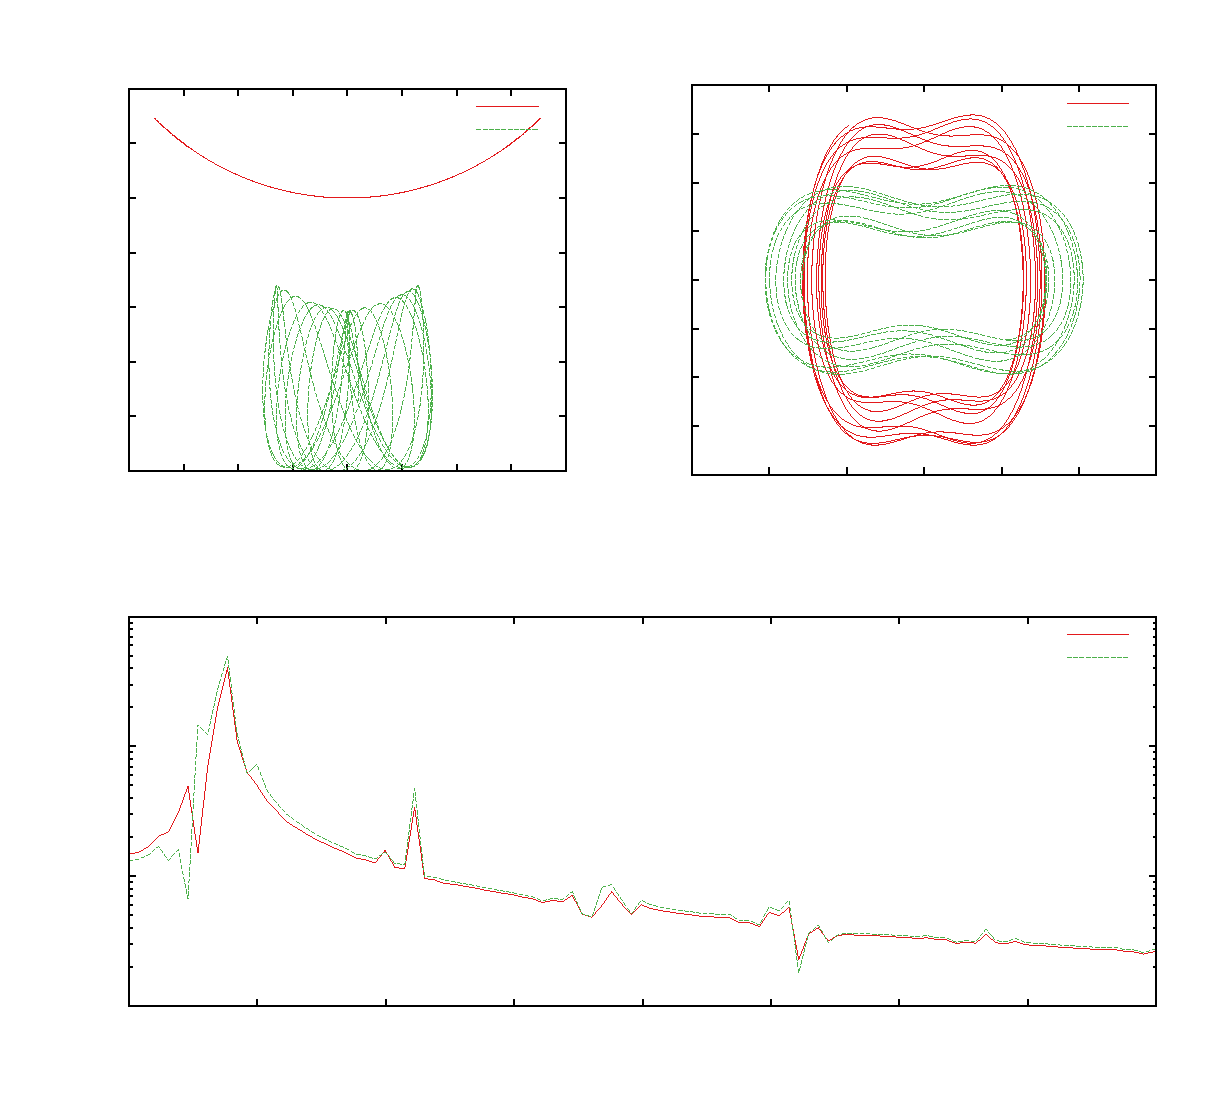
\includegraphics{./figures/trajektorie5}}%
    \gplfronttext
  \end{picture}%
\endgroup
}
\caption{Doppelpendel über einen Zeitraum von $t = \num{16.4} \, \si{\second}$ in Schritten von $h = \num{0.001} \, \si{\second}$. Anfangsbedingung: $\theta_1 = \frac{\pi}{4}$, $\theta_2 = -\frac{\pi}{4}$, $\omega_1 = \omega_2 = \num{0} \, \si{\per\second}$.}
\label{fig5}
\end{figure}

\end{document}
